%Appendix
\section{Details of Stretcher Design}

Aluminum was chosen as the base material because of its sturdy yet malleable nature, making it an excellent material with which to mill. Acrylic was considered, but was not chosen because of its brittle nature; we were concerned about cracking when drilling the UNF threads connecting to the Luer-lock syringe.

The stretched sheet is laid over the lubricated apparatus and fixed in place using a 48.7mm diameter by 1.6mm thick rubber O-ring. A removable plastic ring is then placed on top of the o-ring and clamped down using a tension clamp attached to a fitted plastic base slotted for the stretching apparatus to sit. The plastic ring is constructed from an engineering plastic that came from a similar but malfunctioning device used by our colleagues at ETH Zürich. The outer ring could easily be laser cut from a plastic or milled out of aluminum if desired. 

To pull a vacuum, a 1/4-28 UNF to female Luer connects the apparatus to a plastic 100ml Luer-lock syringe. We found a more consistent stretch was held by lining the inner walls of the syringe in more Dow Corning vacuum grease. The UNF to female Luer connector is stainless steal, and coated with Dow Corning vacuum grease. The inclusion of a small o-ring between the UNF threads and the cylindrical base proved critical in holding vacuum for sustained periods of time.

The vacuum pull was controlled by a Harvard Apparatus Elite 11 Syringe Pump. This allows us to have a consistent withdraw rate and control over the amount of air withdrawn down to the pico-liter level, a far ggreater precision than needed. Stretching was found to work best at maximum withdrawal rate. Our stretching apparatus has sustained a constant equibiaxial stretch at 36\% strain for as long as 5 hours. Maximum strain percentage and during of maintained stretch is yet to be fully tested.


\begin{figure}[h!]	
	%\centering centers the figure on the page.  This is convention.

	\vspace{-3.7em}
	\centerline{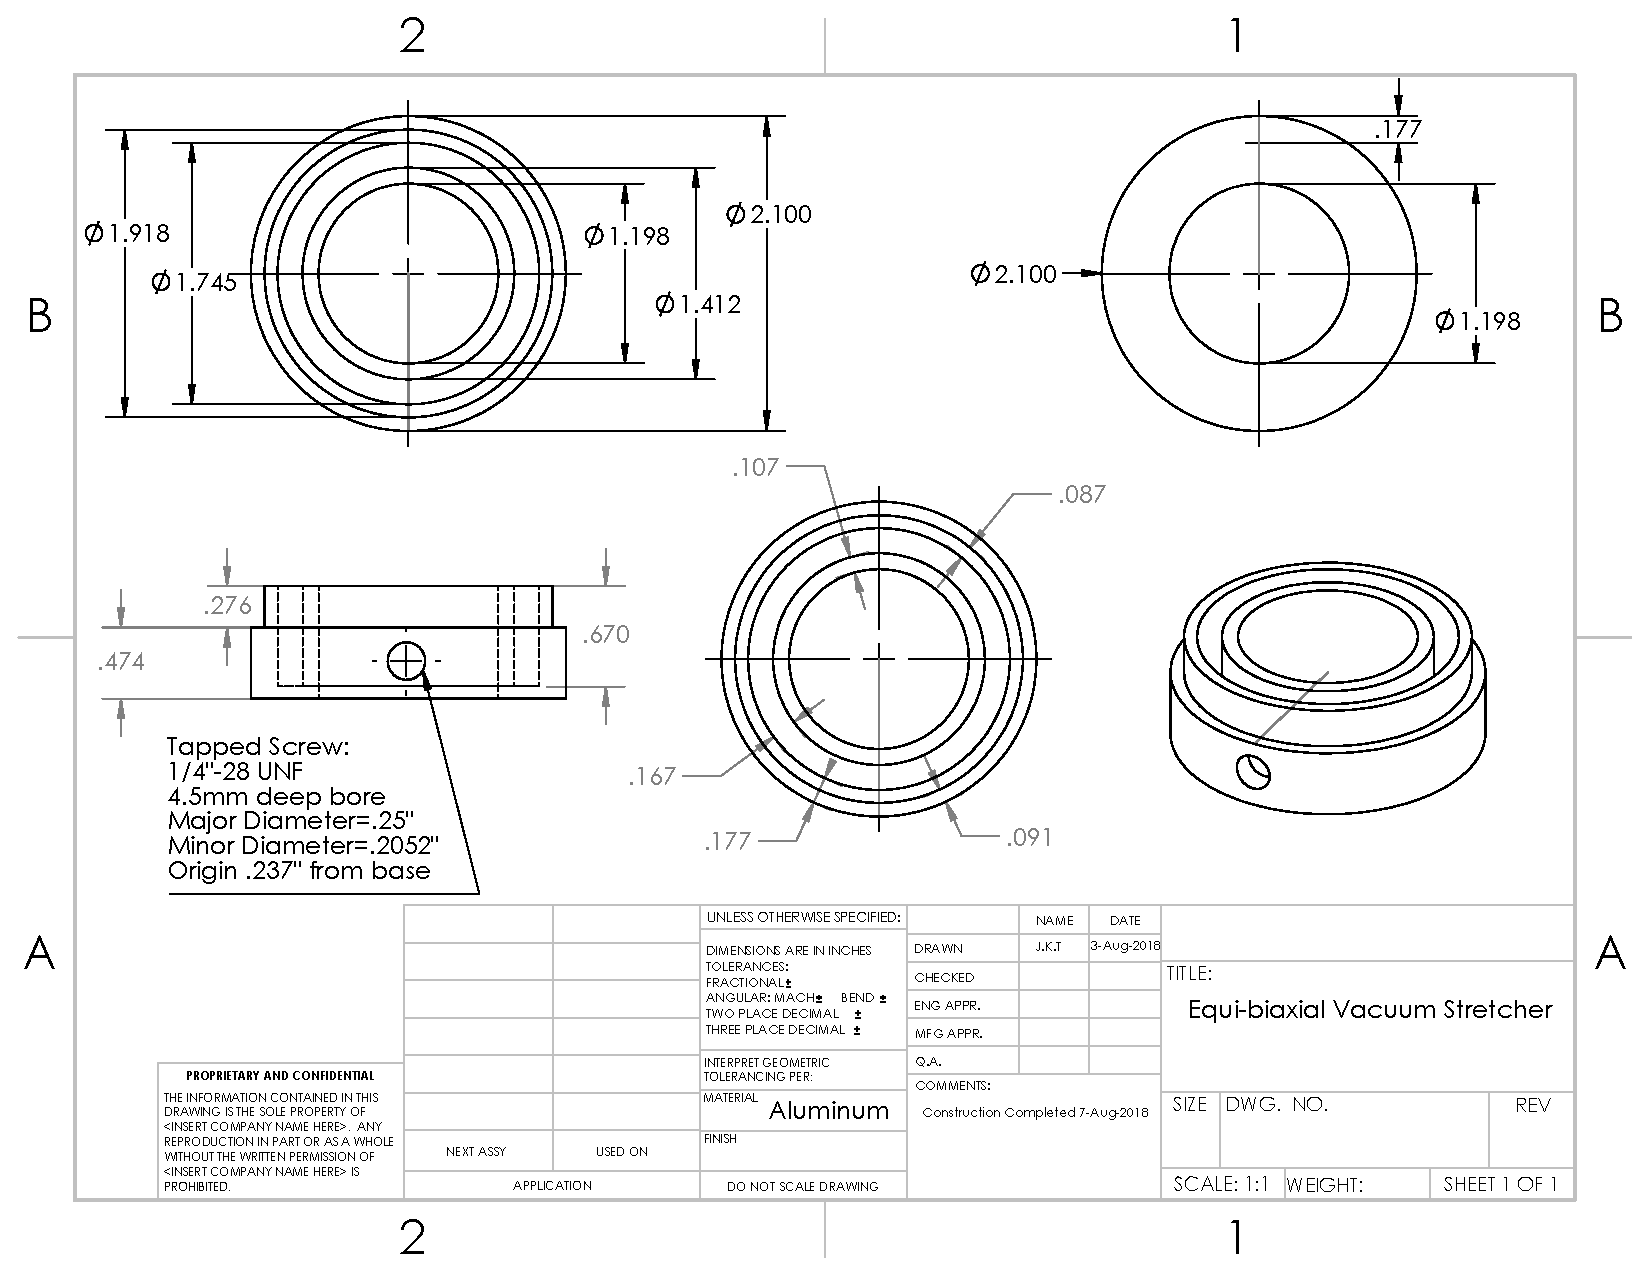
\includegraphics[scale=.65]{Chapters/Figures/Stretcher_body_with_screwtap_updated.PDF}}
	 
	\caption[Stretching Apparatus Design Document]{The equi-biaxial vacuum stretcher design document. Note: all measurements are in inches.}
	
%	This reference can be called in the text using the \ref tag.
	\label{fig:stretcherDesignBase}
\end{figure}


\begin{figure}[h!]
	%\centering centers the figure on the page.  This is convention.
	
	
	\centerline{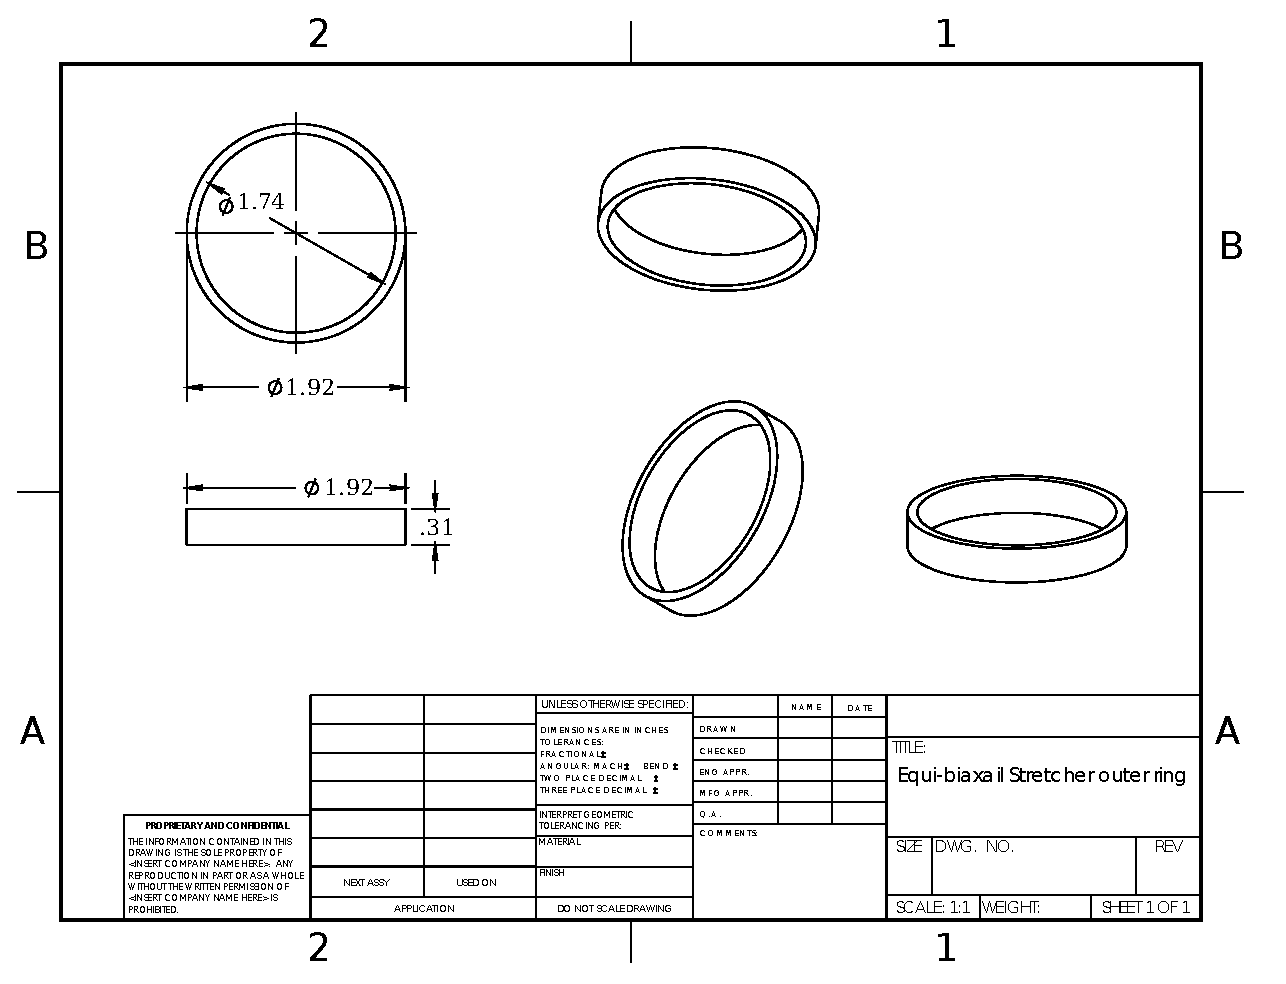
\includegraphics[scale=.85]{Chapters/Figures/Stretcher_outer.pdf}}
	\vspace{-.7em}
	\caption[Stretcher outer-ring]{Engineering Design Document of the outer-ring for the Stretching Apparatus. Note: all measurements are in millimeters.}
	
	%	This reference can be called in the text using the \ref tag.
	\label{fig:stretcherDesignRing}
\end{figure}

%Appendices are a good idea for almost any thesis.  Your main thesis body will likely contain perhaps 40-60 pages of text and figures.  You may well write a larger document than this, but chances are that some of the information contained therein, while important, does \emph{not} merit a place in the main body of the document.  This sort of content - peripheral clarifying details, computer code, information of use to future students but not critical to understanding your work \ldots - should be allocated to one or several appendices.  
